%\documentclass{article} % For LaTeX2e
% Optional math commands from https://github.com/goodfeli/dlbook_notation.
%% Recurrent neural networks have been widely used for processing sequences. Recurrent neural networks are known for their exploding and vanishing gradient problem (EVGP). This problem becomes more evident in tasks where the information needed to correctly solve them exist over long time scales, because
%% EVGP prevents important gradient components from being back-propagated adequately over a large number of steps. This paper aims to reproduce the results of the paper \cite{kanuparthi2018hdetach}. \cite{kanuparthi2018hdetach}  introduces a stochastic algorithm (h-detach) to mitigate the EVGP problem in Long Short Term Memory networks. Long Short Term Memory networks – usually just called “LSTMs” – are a special kind of RNN, capable of learning long-term dependencies.

\vspace{-2em}

\section{Introduction}

Recurrent neural networks\supercite{Rumelhart:1988:LRB:65669.104451} are widely used for processing sequences of information. Recurrent neural networks are very hard to optimize due to the exploding and vanishing gradient problem \cite{pmid:18267787}. This problem becomes more evident in tasks where training data has dependencies that exist over long time scales. A number of architectures have been proposed to mitigate this problem. These architectures include Long Short Term Memory\supercite{Hochreiter:1997:LSM:1246443.1246450}, Gated Recurrent Unit\supercite{DBLP:journals/corr/ChungGCB14}. These networks introduce a linear temporal path that allow gradients to flow freely across time-steps. The LSTM is the most widely used architecture. It has been shown that LSTMs have greater representational power as compared to the other architectures\supercite{DBLP:journals/corr/abs-1805-04908}. It is still hard to optimize LSTMs to learn long term dependencies.

The authors say that when the weights of the LSTM are large, the gradients through the linear temporal path get suppressed. This path is important as it was introduced to carry information about long term dependencies. The authors prove this empirically. To prevent this, the authors provide a simple stochastic algorithm (h-detach). The authors experiment with this algorithm on tasks that require capturing long-term dependencies. Examples of such tasks include the copying task\supercite{pmid:18267787,DBLP:journals/corr/abs-1211-5063} and the sequential-mnist task\supercite{DBLP:journals/corr/LeJH15}. The authors claim that their approach results in faster convergence and stable training. In this work, we attempt to reproduce the results for the copying task and the sequential mnist task (permuted and non-permuted). We also conduct experiments to prove their claims mentioned in the ablation study.


\section{Proposed Method:H-detach}
We will first introduce the LSTM equations and then analyze the problems with back-propagation according to the authors.

\subsection{Long Short Term Memory Networks}
LSTM was introduced to provide free-flowing paths for gradients to propagate. The equations of the LSTM can be defined as follows-
\begin{center}
    \begin{equation}\label{eq1}
         c_t=f_t \odot c_{t-1} + i_t \odot g_t
    \end{equation}
   
\end{center}

\begin{center}
    \begin{equation} \label{eq2}
    h_t=o_t \odot \tanh(c_t)    
    \end{equation}
    
\end{center}

Here, $\odot$ denotes the pointwise product and the gates $f_t$, $i_t$, $g_t$ and $o_t$ are defined as

\begin{equation} \label{eq3}
 f_t=\sigma(W_{fh}h_{t-1}+W_{fx}x_{t}+b_f)    
 \end{equation}
 \begin{equation} \label{eq4}
 i_t=\sigma(W_{ih}h_{t-1}+W_{ix}x_{t}+b_i)    
 \end{equation}
 \begin{equation} \label{eq5}
    g_t=\tanh(W_{gh}h_{t-1}+W_{gx}x_{t}+b_g)    
    \end{equation}
    \begin{equation} \label{eq6}
    o_t=\sigma(W_{oh}h_{t-1}+W_{ox}x_{t}+b_o)    
    \end{equation}

Here, $c_t$ and $h_t$ are the cell state and hidden state respectively. The output of the LSTM at each time step is $\phi$($h_t$). The loss is calculated as $l_t=l(\phi(h_t))$. In an auto-regressive LSTM networks,the output of one time step is fed as input to the next time step. There is a linear recursive relation between the cell states $c_t$. This path is the linear temporal path which allows the free flowing of gradients backwards. More information about LSTMs can be obtained from \href{http://colah.github.io/posts/2015-08-Understanding-LSTMs/}{colah's blog}.


\subsection{Backpropagation}
Here we will present the authors analysis of the backpropagation equations in brief. Let w be a weight in one of the weight matrices ($W_{fh}$,$W_{fx}$,$W_{ih}$,$W_{ix}$,$W_{gh}$,$W_{gx}$,$W_{oh}$ or $W_{ox}$). Let,


    \begin{equation} \label{eq7}
        z_t=\begin{vmatrix}
             dh_t/dw  \\
             dc_t/dw \\
             1_n
        \end{vmatrix}
    \end{equation}


Then, $z_t=(A_t+B_t)z_{t-1}$. The exact definitions of $A_t$ and $B_t$ can be obtained from \cite{kanuparthi2018hdetach}. The equation for $z_t$ can be expanded as 
    \begin{equation} \label{eq8}
        z_t=(A_t+B_t)(A_{t-1}+B_{t-1})...(A_2+B_2)z_1
    \end{equation}
Here $A_t$ carries the gradients that arise due to the linear temporal path. The matrix $A_t$ is bounded given that the number of time steps is finite and the initialization of $c_0$ is finite. On the other hand, the matrix $B_t$ is obtained through the repeated multiplication of weights. If the weights are large, the matrix $B_t$ can also become very large in magnitude. In this case, the magnitude of $A_t$ will be very small as compared to $B_t$, hence the gradients through the linear temporal path (which carry information of long term dependency) will have no effect on the weights.

\subsection{Algorithm : h-detach}

The above problem can be mitigated by multiplying $B_t$ by a positive number between 0 and 1. The authors provide a simple stochastic algorithm to achieve this which is presented as Algorithm~\ref{alg1}.

\begin{algorithm}
\caption{h-detach algorithm}\label{alg1}
\begin{algorithmic}[1]
\State \textbf{Input} : $p$, $h_0$, $c_0$, [$x_0$,$x_1$,.....,$x_T$]
\State $l\gets 0$
\For{$1\leq t \leq T$}
\If{$bernoulli(p)== 1$}
\State $\tilde{h}_{t-1}\gets stop\_gradient(h_{t-1})$
\Else
\State $\tilde{h}_{t-1}\gets h_{t-1}$
\EndIf
\State $h_t,c_t \gets LSTM(x_t,\tilde{h}_{t-1},c_{t-1})$
\State $l_t \gets L(\phi(h_t))$
\State $l \gets l + l_t$
\EndFor
\State \textbf{return} $l$

\end{algorithmic}
\end{algorithm}



\section{Implementation Details}

The authors have made their code public\footnote{\url{https://github.com/bhargav104/h-detach}}. The codebase used for the reproducibility experiments is also publicly available\footnote{\url{https://github.com/dido1998/h-detach}}.The implementation is in Pytorch\footnote{\url{https://pytorch.org/}}. The author provides instructions to run the code to perform the experiments. We could get the code running immediately without any changes. The stop-gradient in algorithm~\ref{alg1} can be implemented using the detach()\footnote{\url{https://pytorch.org/docs/stable/autograd.html\#torch.Tensor.detach}} method in pytorch. 

The authors claim that LSTMs trained using h-detach converge in lesser number of epochs as compared to normal LSTMs. We have been able to confirm this claim in our experiments. Even though the convergence is faster in terms of the number of epochs, the implementation (provided by the authors) is slower as compared to the vanilla LSTM implementation provided by pytorch \footnote{\url{https://pytorch.org/docs/stable/nn.html\#torch.nn.LSTM}}. This is because, in the implementation, each input is fed sequentially which makes it slower compared to feeding inputs at all time steps at once (as is usually done for efficiency). On communication with the authors, it was confirmed that this was done to ensure the correctness of the h-detach algorithm. The authors have themselves implemented the LSTM cell in pytorch. In our experiments, we observed that implementing the LSTM cell in CUDA code. The code can be found in the reproducibility repo\footnote{\url{https://github.com/dido1998/h-detach/tree/master/h-detach-cuda-extension}}. Implementing the LSTM cell in CUDA code can result in upto 2x speed-up. This CUDA code can be added as an extension in pytorch and used.



\section{Experiments}
\label{others}

\subsection{Copying Task}

This task requires the recurrent network to memorize the network inputs provided at the first few
time steps and output them in the same order after a large time delay.  Thus the only way to solve
this task is for the network to capture the long term dependency between inputs and targets which
requires gradient components carrying this information to flow through many time steps.
The authors define 10 token $\{a_i\}^{i=9}_{i=0}$. The input to the LSTM is a sequence of length T + 20 formed using one of the ten tokens at each time step. Input for the first 10 time steps are sampled i.i.d. (uniformly) from $\{a_i\}^{i=7}_{i=0}$. The next T−1 entries are set to $a_8$, which constitutes a delay. The next single entry is $a_9$,  which represents a delimiter,  which should indicate to the algorithm that it is now required to reproduce the initial 10 input tokens as output. The remaining 10 input entries are set to $a_8$.  The target sequence consists of $T+ 10$ repeated entries of $a_8$, followed by the first 10 entries of the input sequence in exactly the same order. This copying task is similar to the one described in \cite{DBLP:journals/corr/ArjovskySB15}.
We run each experiment for 200-300 epochs. The main point the authors wanted to prove is that using h-detach results in more stable training and faster convergence. We observe that these properties can be observed in the first 200-300 epochs. The authors have used the probability values of 0.25 and 0.50 for h-detach. The original paper does not mention how they arrived at these values. However, on the openreview site\footnote{\url{https://openreview.net/forum?id=ryf7ioRqFX}}, the authors mention that they tried the probability values 0.1, 0.25, 0.4, 0.5, 0.75 and 0.9. They found that the values between 0.25 and 0.50 work the best. \\

We present our experiments in Figure ~\ref{fig1:figure1}. The top row presents results for the copying task with T=100 and with the probabilities for h-detach set as 0, 0.25 and 0.5. The bottom row presents results for the copying task with T=300 and the same probabilities. As the authors mention, we see the main advantage of using h-detach in the task with T=300. We see that, the models trained with h-detach result in higher accuracies and faster convergence. Here, we also see that p=0.50 works better than p=0.25. For the task with T=100, we observe that both methods achieve high accuracy of close to ~100\% but h-detach results in faster convergence. The hyperparameters are exactly the same as  provided by the authors in the source code.


\begin{figure}[ht]
\begin{center}
  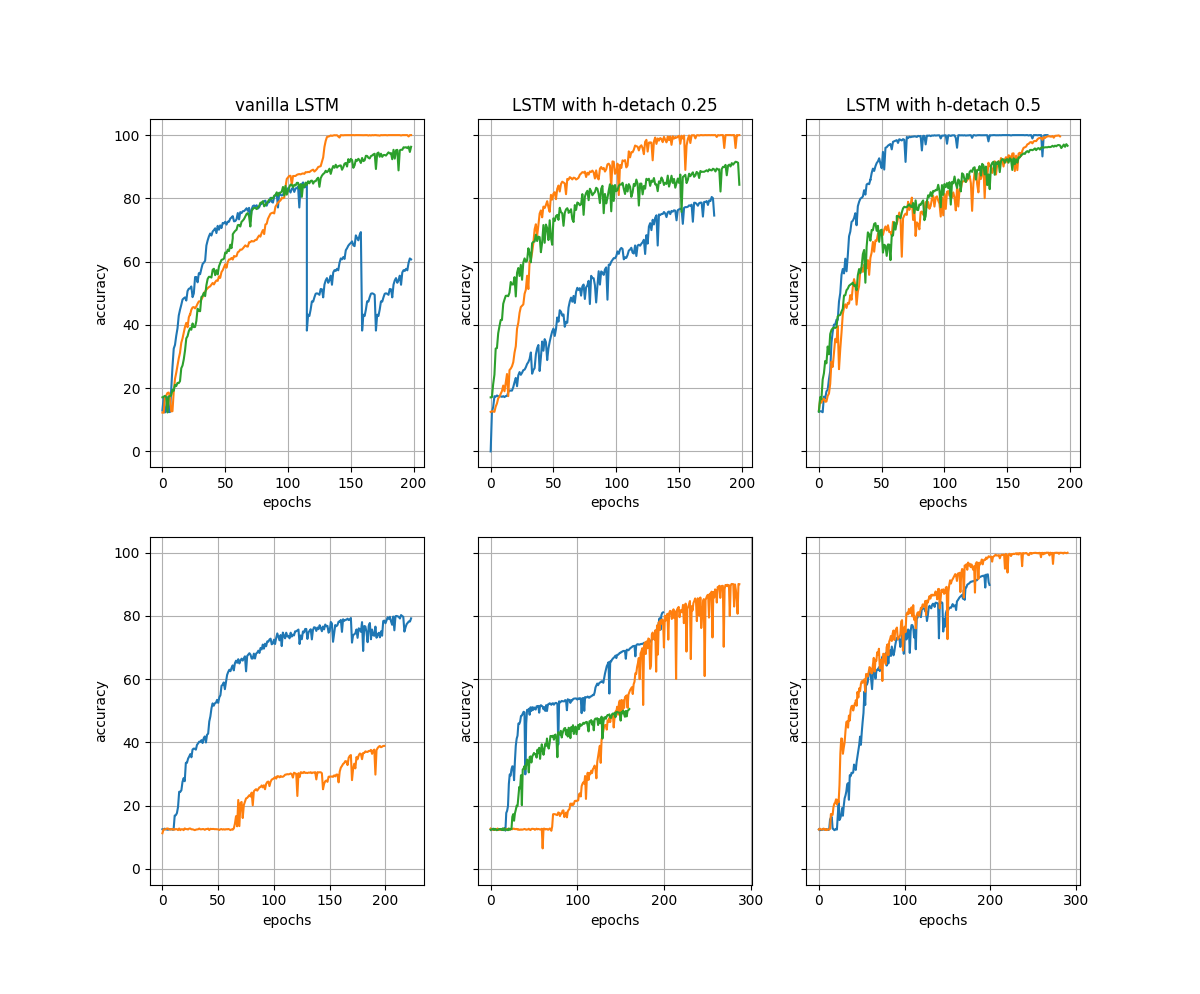
\includegraphics[width=\linewidth,height=6cm]{figures/h_detach_new.png}
\end{center}
\caption{Validation accuracy curves for vanilla LSTM (left), h-detach with probability 0.25 (centre) and h-detach with probability 0.5(right) for the copying task. The top row shows the curves for T=100 and the bottom row shows the curves for T=300. For T=300, we can see that only the LSTMs with h-detach are able to cross the accuracy of 80\%. It can be seen that training with h-detach is more stable and leads to faster convergence. Each experiment was tried with two different seeds.}
\label{fig1:figure1}
\end{figure}


\subsection{Sequential MNIST}
This is the sequential version of the MNIST classification task. Each pixel is fed one at a time. The authors consider two versions of this task: one is which the pixels are fed in order (left to right and top to bottom) and the other is in which pixels are fed in random but fixed order. The second one is called permuted mnist. We tested with two different learning rates (0.0005 and 0.001). The results can be seen in Figure ~\ref{figure2}

\begin{figure}[ht]
\begin{center}
%\framebox[4.0in]{$\;$}
 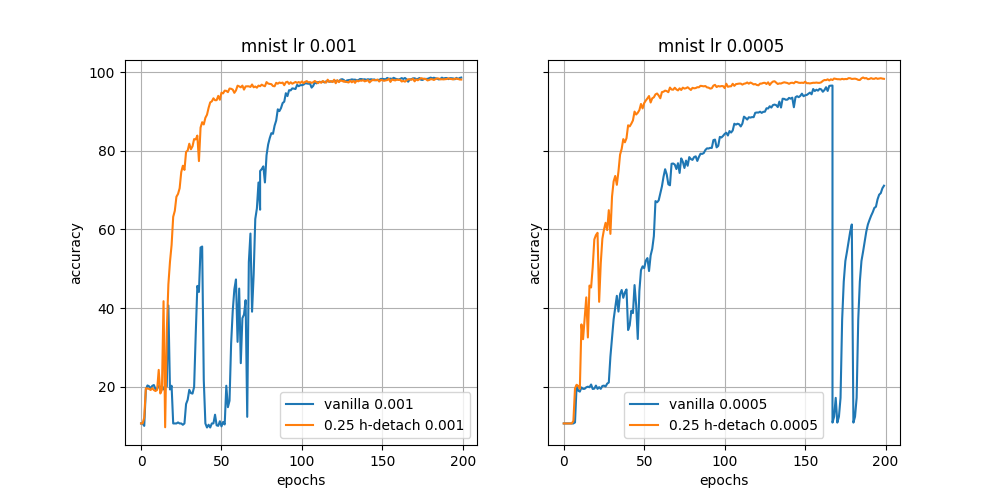
\includegraphics[width=\linewidth, height = 4cm]{figures/mnist.png}
\end{center}
\caption{Validation accuracy curves for the sequential mnist task. Each plot shows the accuracy curves with and without h-detach for different learning rates. H-detach is more robust to different learning rates and converges faster.}
\label{figure2}
\end{figure}

The optimizer used was ADAM. The batch-size was set to 100. The number of examples in the training set was set to 50000, 10000 for validation and 10000 for testing. The number of epochs was set to 200. On the sequential MNIST task, vanilla LSTM and training with h-detach give an accuracy of 98.60\%(authors report 98.60\%) and 98.62\%(authors report 98.80\%) respectively. The numbers are not very different but we observed that training with h-detach gives faster convergence.
For the permuted mnist (pmnist) task we trained with h-detach and obtained the maximum accuracy of 91.96\%(authors report 92.92\%). The validation accuracy curve for the permuted mnist task can be found in Figure~\ref{figure4}



\begin{figure}[h]
\begin{center}
%\framebox[4.0in]{$\;$}
 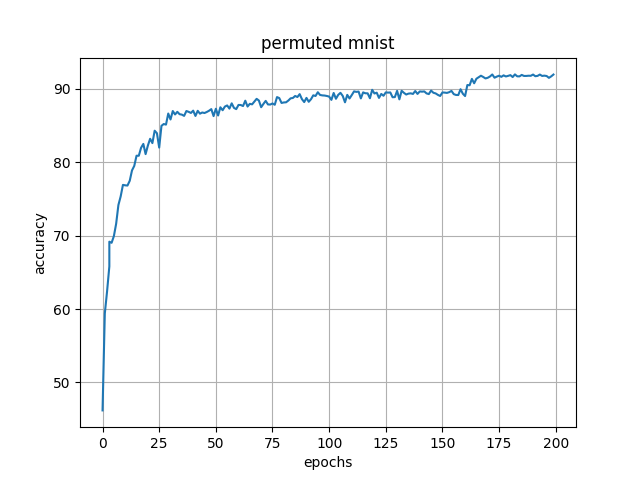
\includegraphics[width=\linewidth,height=4cm]{figures/pmnist.png}

\end{center}
\caption{validation accuracy curve for permuted mnist with h-detach probability 0.25 and learning rate 0.001.}
\label{figure4}
\end{figure}


\subsection{Ablation Studies}
The authors first study the effect of removing gradient clipping from the sequential mnist task. This would be insightful as it would confirm that stochastically blocking gradients through the hidden state $h_t$ prevents increase in gradient magnitude. As the authors say, we observe that removing gradient clipping makes the training extremely unstable in the case of a vanilla LSTM as compared to LSTM with h-detach.This is demonstrated in Figure~\ref{figure5}.

\begin{figure}[ht]
\begin{center}
%\framebox[4.0in]{$\;$}
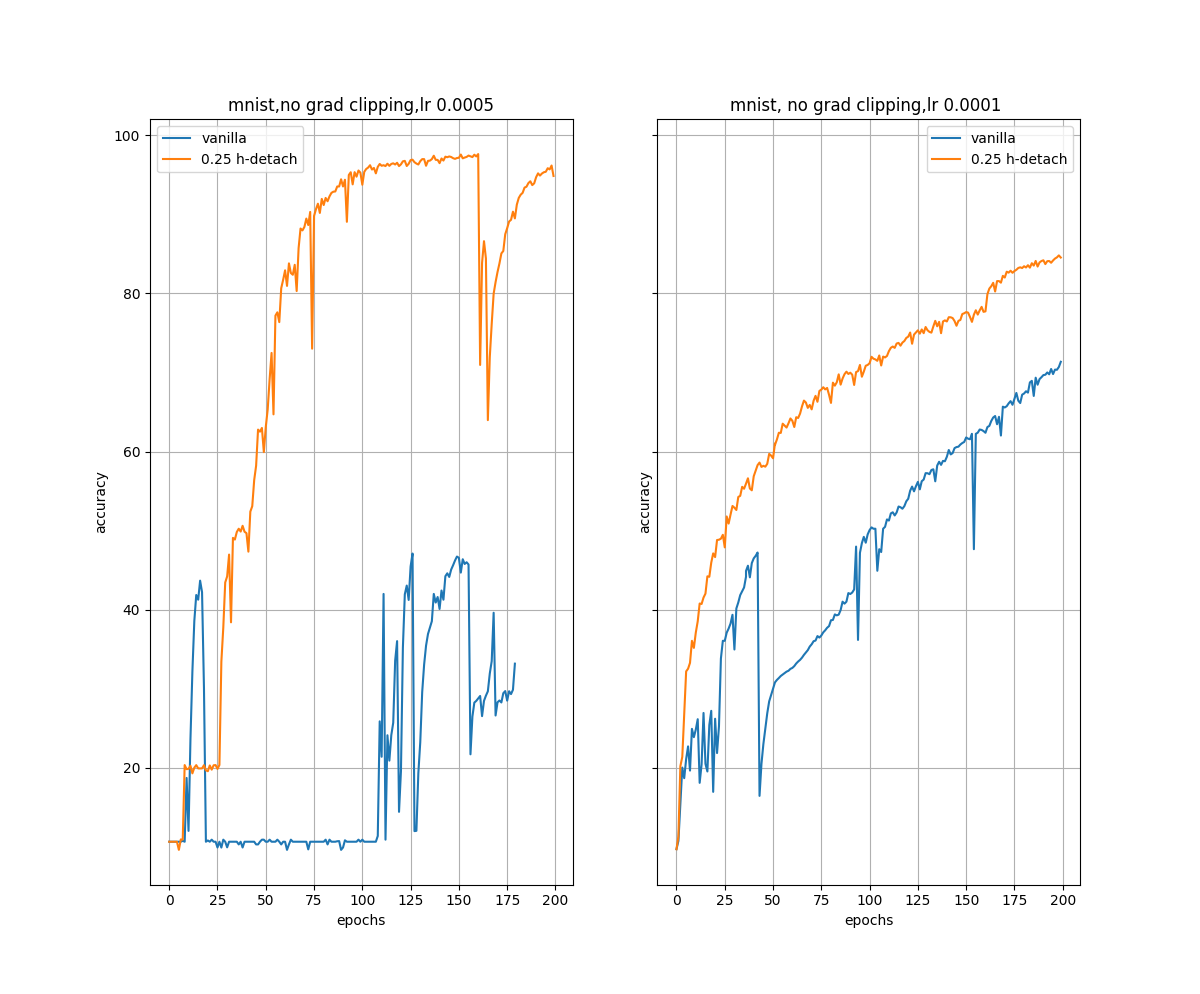
\includegraphics[width=\linewidth,height=6cm]{figures/gradclip22.png}
\end{center}
\caption{The effect of removing gradient clipping while training for vanilla LSTM vs LSTM with h-detach.}
\label{figure5}
\end{figure}

The authors also conduct experiments to prove that the cell state carries information about long term dependencies. This is done by stochastically blocking gradients through the cell state instead of the hidden state. This new algorithm is tested on the copying task with T=100 and the sequential mnist task. The results are demonstrated in Figure~\ref{figure6}. For the copying task, the accuracy does not cross 40\% even after 200 epochs. For the sequential mnist task, the accuracy crosses 80\% but the training is extremely unstable and the h-detach version completely out performs the c-detach version.


\begin{figure}[ht]
\begin{center}
%\framebox[4.0in]{$\;$}
 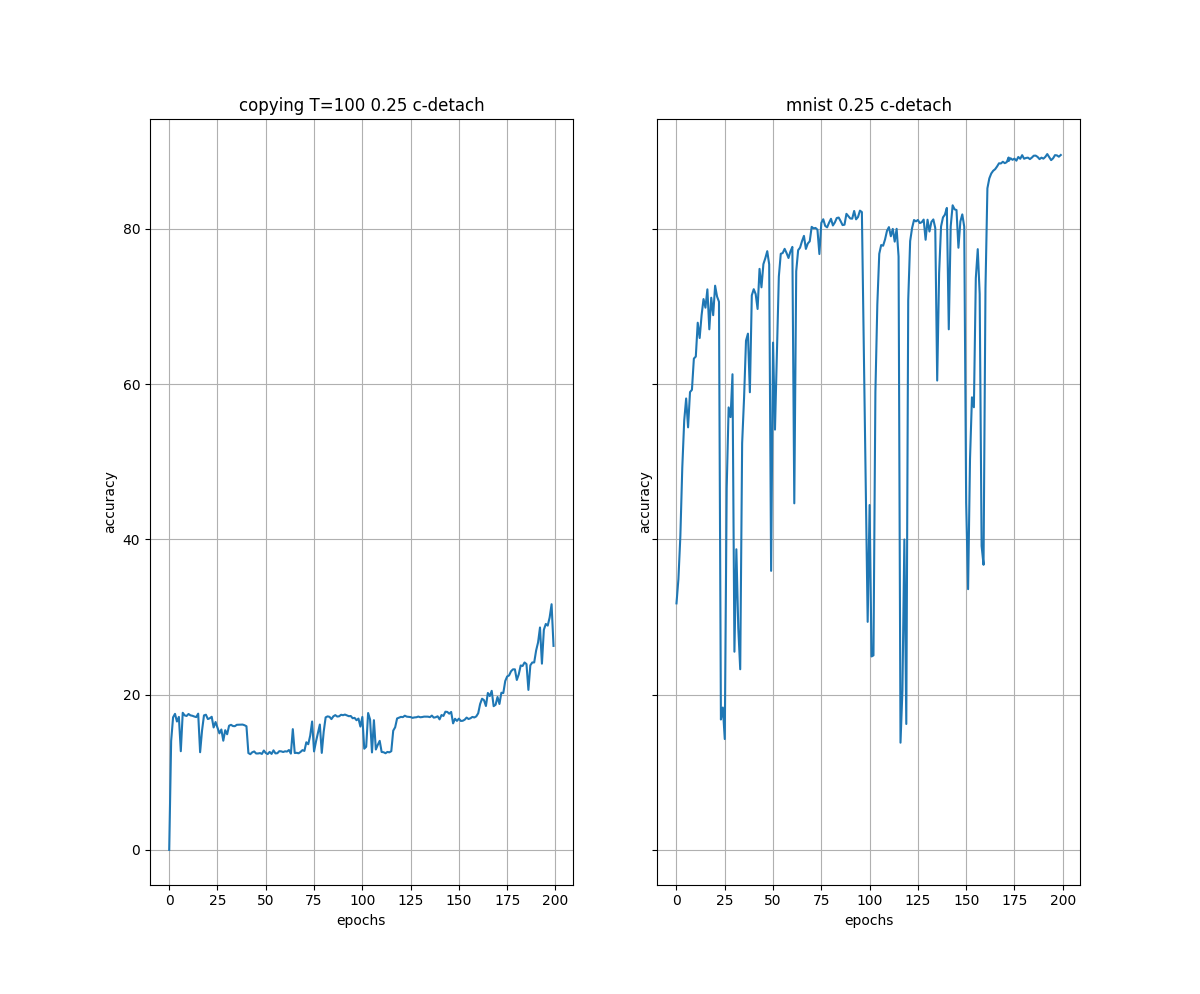
\includegraphics[width=\linewidth,height=6cm]{figures/c_detach.png}
\end{center}
\caption{Validation accuracy curves for the copying task T=100(left) and pixel mnist task(right) such that the gradient is stochastically blocked through the cell state(c-detach). The highest accuracy obtained for the pixel mnist task is 89.65\%. As the authors say, c-detach performs worse than vanilla LSTM. This proves that the cell state path carries information about long term dependencies. }
\label{figure6}
\end{figure}
\section{Environment details}

The experiments were conducted on a NVIDIA GTX 1060 and on google colab\footnote{\url{https://colab.research.google.com/}} (tesla K80).

\section{Future work}

Though the authors have thoroughly explored the advantages of the h-detach algorithm through their experiments, they have not evaluated their proposed algorithm on stacked LSTM networks and bidirectional RNNs with LSTM cells. It would be interesting to see if we get similar performance improvements on these architectures as in the single layer uni-directional case.


\section{Conclusion}
In this paper, we reproduce selected experiments of the original paper, \cite{kanuparthi2018hdetach}. Through communication with the authors, we understood that the main aim of this work was to prove that h-detach achieves better training stability, convergence speed, and it is robust to different learning rates and seeds. Though some of the numbers reported do not match exactly with the original paper, we have successfully proved that h-detach results in more stable and faster convergence. 

